\chapter{Gas Electron Multiplier Detectors}
\label{chap:II-1-gem}

  In 1968, G. Charpak revolutionized the field of tracking detectors by introducing the Multiwire Proportional Chamber (MWPC). MWPCs were more reliable than the existing single-wire gas counters providing a higher sub-mm resolution and rate capabitilies up to fluxes of several MHz cm$^{-2}$. Developments of manufacturing technics and high-density electronics led to a new generation of detectors fulfilling the needs of high-energy physics experimentation. However, their use in high-luminosity experiments revealed some intrensic weaknesses: the mechanical design of the chamber limits the spacial resolution; long ion drift times affect the efficiency of the detector at high fluxes; solid deposits aglomerate on the wires due to aging and induce sparks in the chamber. \\

  Twenty years later, Micro-Strip Gas Counters (MSGCs) were developped using photolithographic processes to engrave anode and cathode strips on an insulating support. Both the position resolution and the rate capability were increase by several orders of magnitude. Unfortunalty, the detectors were prone to the effect of aging and discharges, irremediably damaging the counters. \\

  The relative success of the MSGCs led to the development of Micro-Pattern Gas Detectors (MPGDs) less suseptible to discharges and offering comparable performances. They make use of micro pattern structures to amplify the signal and reduce the probability of sparks inside the chamber. Two technologies have proven to be operationnal: the micro-mesh gaseous structure (MICROMEGAS) and the Gas Electron Multiplier (GEM) \cite{SAULI1997531}. \\

  Already in use in the COMPASS and TOTEM experiments at CERN, GEM detectors have proven to meet the requirements of high-luminosity environments. In 2009, a dedicated R\&D program was launched to study the feasability of the installation of GEMs in the muon spectrometer of CMS to instrument the positions left vacant by RPCs. Seven years later, the so called GE1/1 muon detector upgrade project has been approved by CMS to be installed during LS2.

  \section{Motivations for the GE1/1 Muon Detector Upgrade}

    During LS2 that will take place in 2018-2019, the CMS GEM collaboration \cite{Colaleo:2021453} will install an additional set of muon detectors in CMS in the 1.6 < |$\eta$| < 2.2 region. The so-called GE1/1 detector will be installed near the ME1/1 CSCs station as shown in Figure \ref{fig:II-1-gem-ge11} which highlights the location of the chamber within the muon spectrometer. \\

    \begin{figure}[h!]
      \centering
      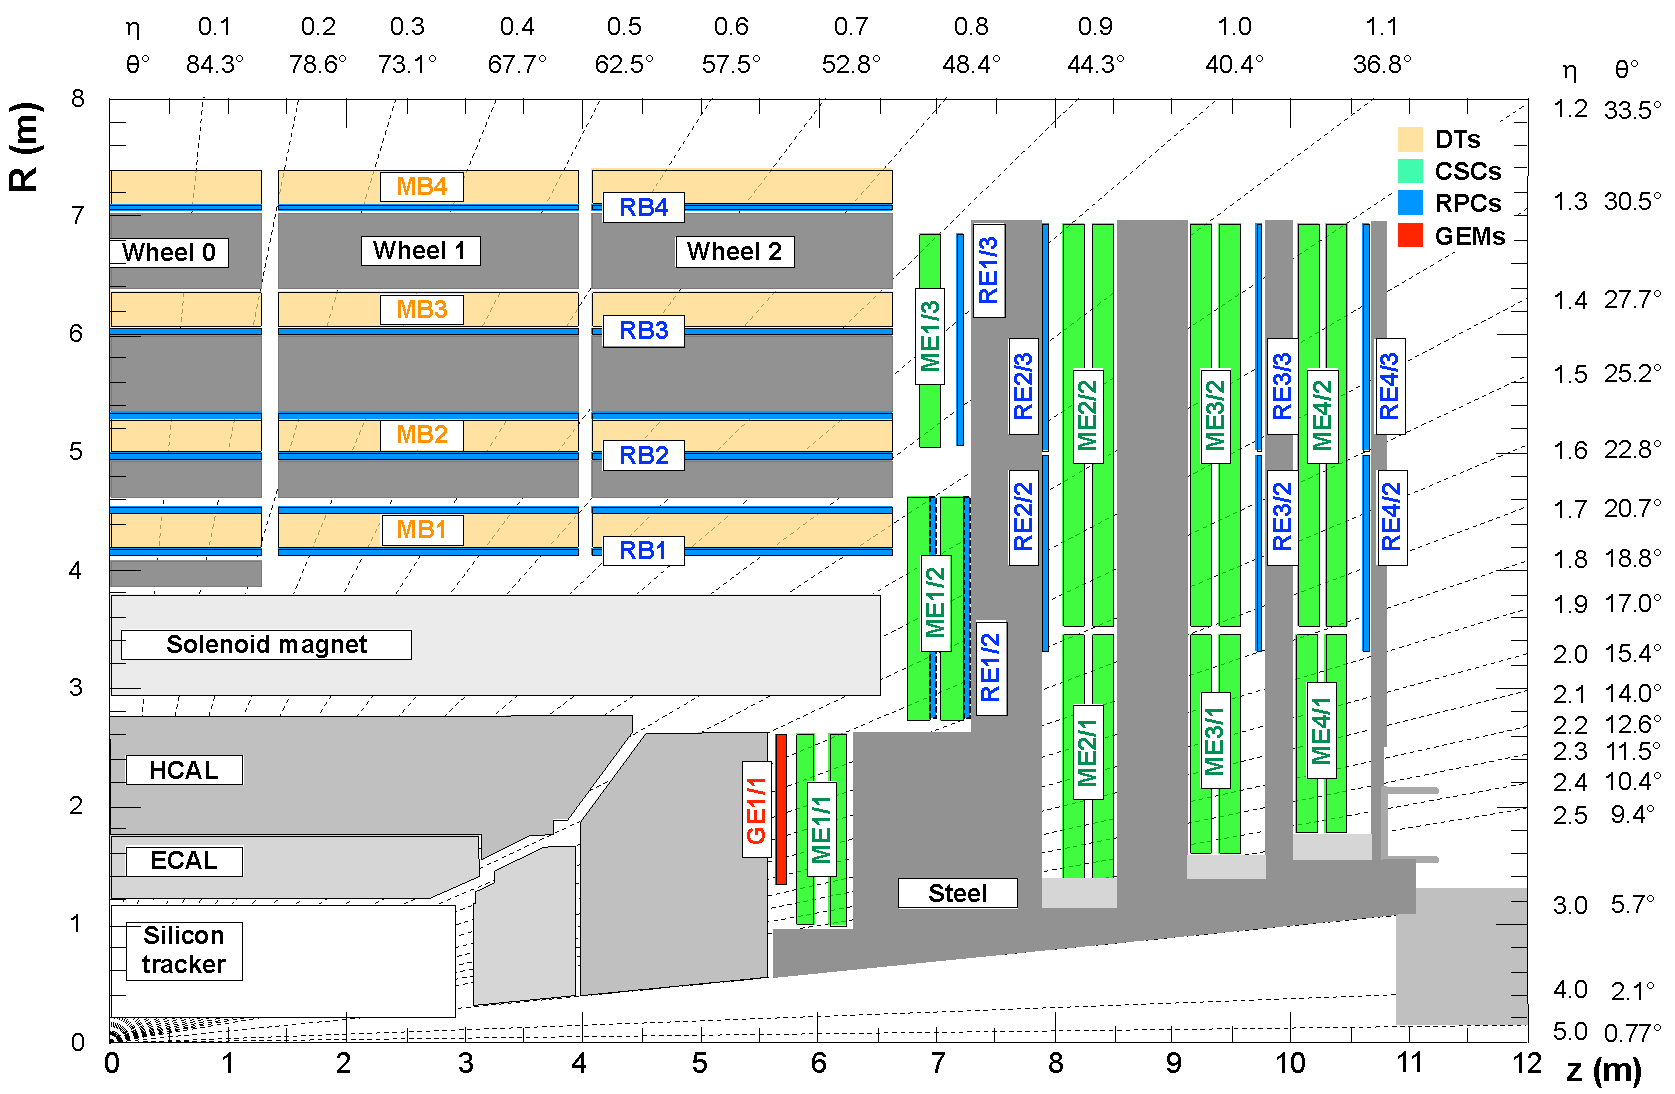
\includegraphics[width=\textwidth]{img/II-1-gem/ge11-quadrant.pdf}
      \caption{Schematic representation of a quadrant of CMS highlighting the location of the GE1/1 detector in red within the muon spectrometer \cite{Colaleo:2021453}.}
      \label{fig:II-1-gem-ge11}
    \end{figure}

    The main motivation for the installation of GE1/1 is the significant impact it has on the triggering system of CMS. Left as is, the performance of the current system would degrade in the coming years with the increase in instantenuous luminosity due to the rate limitations of the ME1/1 station exposed to an intense flux of particles. Muon triggering will in turn suffer a degradation in transverse momentum, p$_T$, resolution. As muon triggers are limited in bandwidth to a fraction of the total allocated bandwidth of the trigger, typically a few kHz, they must set a cut on the minimum p$_T$ of the muons. In the scenario where the muon spectrometer remains unmodified, the threshold would have to be raised to p$_T$ $ \approx $ 30 GeV c$^{-1}$ which would be a considerable drawback in terms of physics analysis. \\

    To prevent the degradation of the trigger system, the GEM collaboration investigated the possibility to use the bending angle of tracks between GE1/1 and ME1/1 to estimate the p$_T$ of muons, which trajectory is curvated by the magnetic field. Figure \ref{fig:II-1-gem-csc-bending} shows on the left the lever arm given by the 20 cm to 46 cm distance between the two detectors. The variation in distance corresponds to "close" and "far" chambers which are staggered in order to allow for some overlap and avoid deadspace. From this, the picture on the right displays the discrimination power between 5 GeV c$^{-1}$ and a 20 GeV c$^{-1}$ muons. \\

    \begin{figure}[h!]
      \centering
      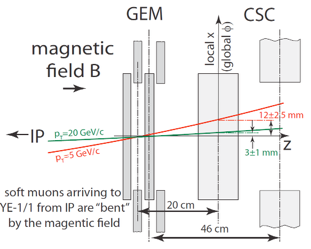
\includegraphics[width=0.45\textwidth]{img/II-1-gem/gem-csc-bending-1.png}
      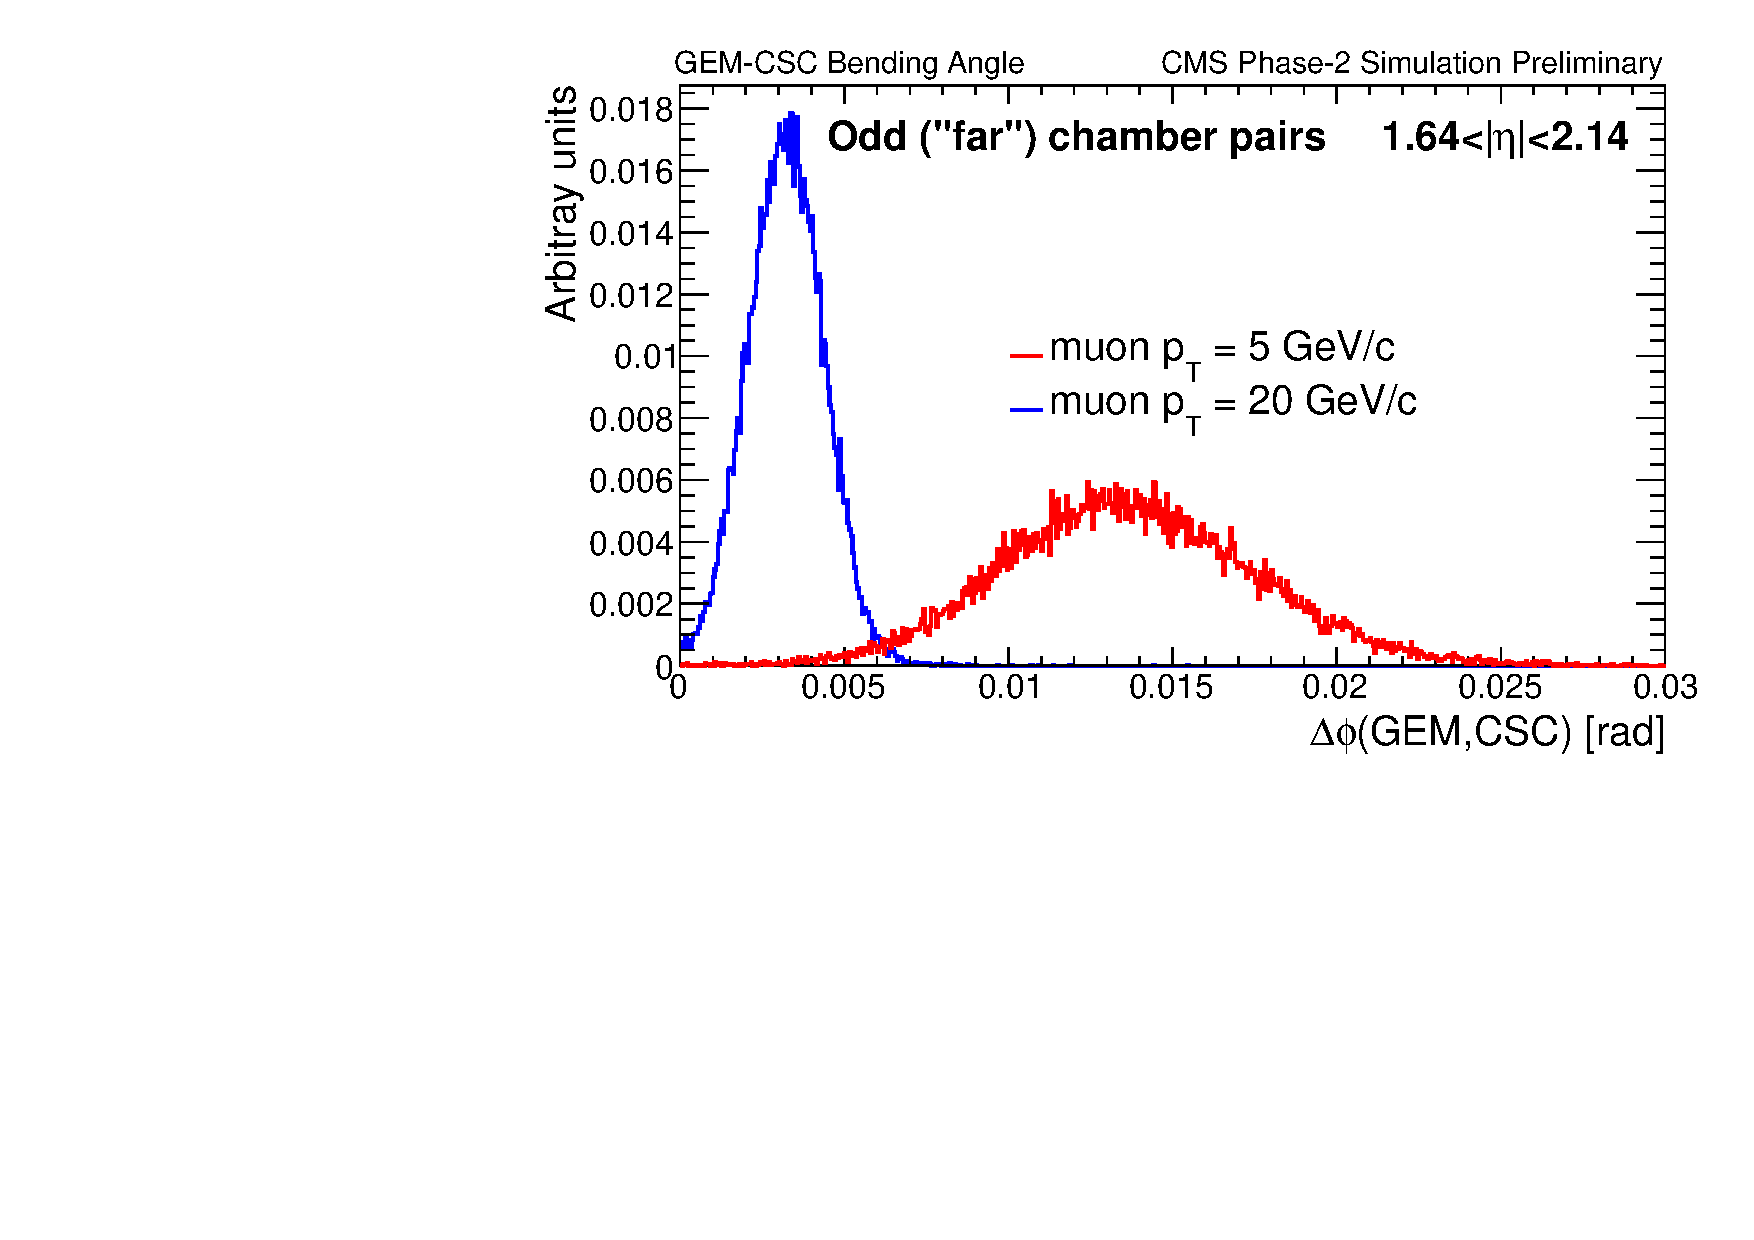
\includegraphics[width=0.53\textwidth]{img/II-1-gem/gem-csc-bending-2.pdf}
      \caption{??? \cite{Colaleo:2021453}.}
      \label{fig:II-1-gem-csc-bending}
    \end{figure}

    Using these results, a common effort from the GEM and CSC collaboration ensued to integrate the GEM measurments in the CSC trigger system to provide an additionnal layer of information. Using simulations, it has been shown that the efficiency of system increases thus yeilding a lower rate of triggers. These results are shown in Figure \ref{fig:II-1-gem-trigger}. In the left plot, it can be seen that the efficiency of the GEM and CSC combined trigger in blue is superior to the CSC only results in red, recovering the losses occuring at higher rates. In the right plot, it is depicted how the trigger rate of the combined system in blue diminishes by one order of magnitude compared to the current system in red. For a given trigger rate, a smaller muon p$_T$ threshold can be applied due to lower rate of misreconstructed particles, which improves the physics performance of the detectors. \\

    \begin{figure}[h!]
      \centering
      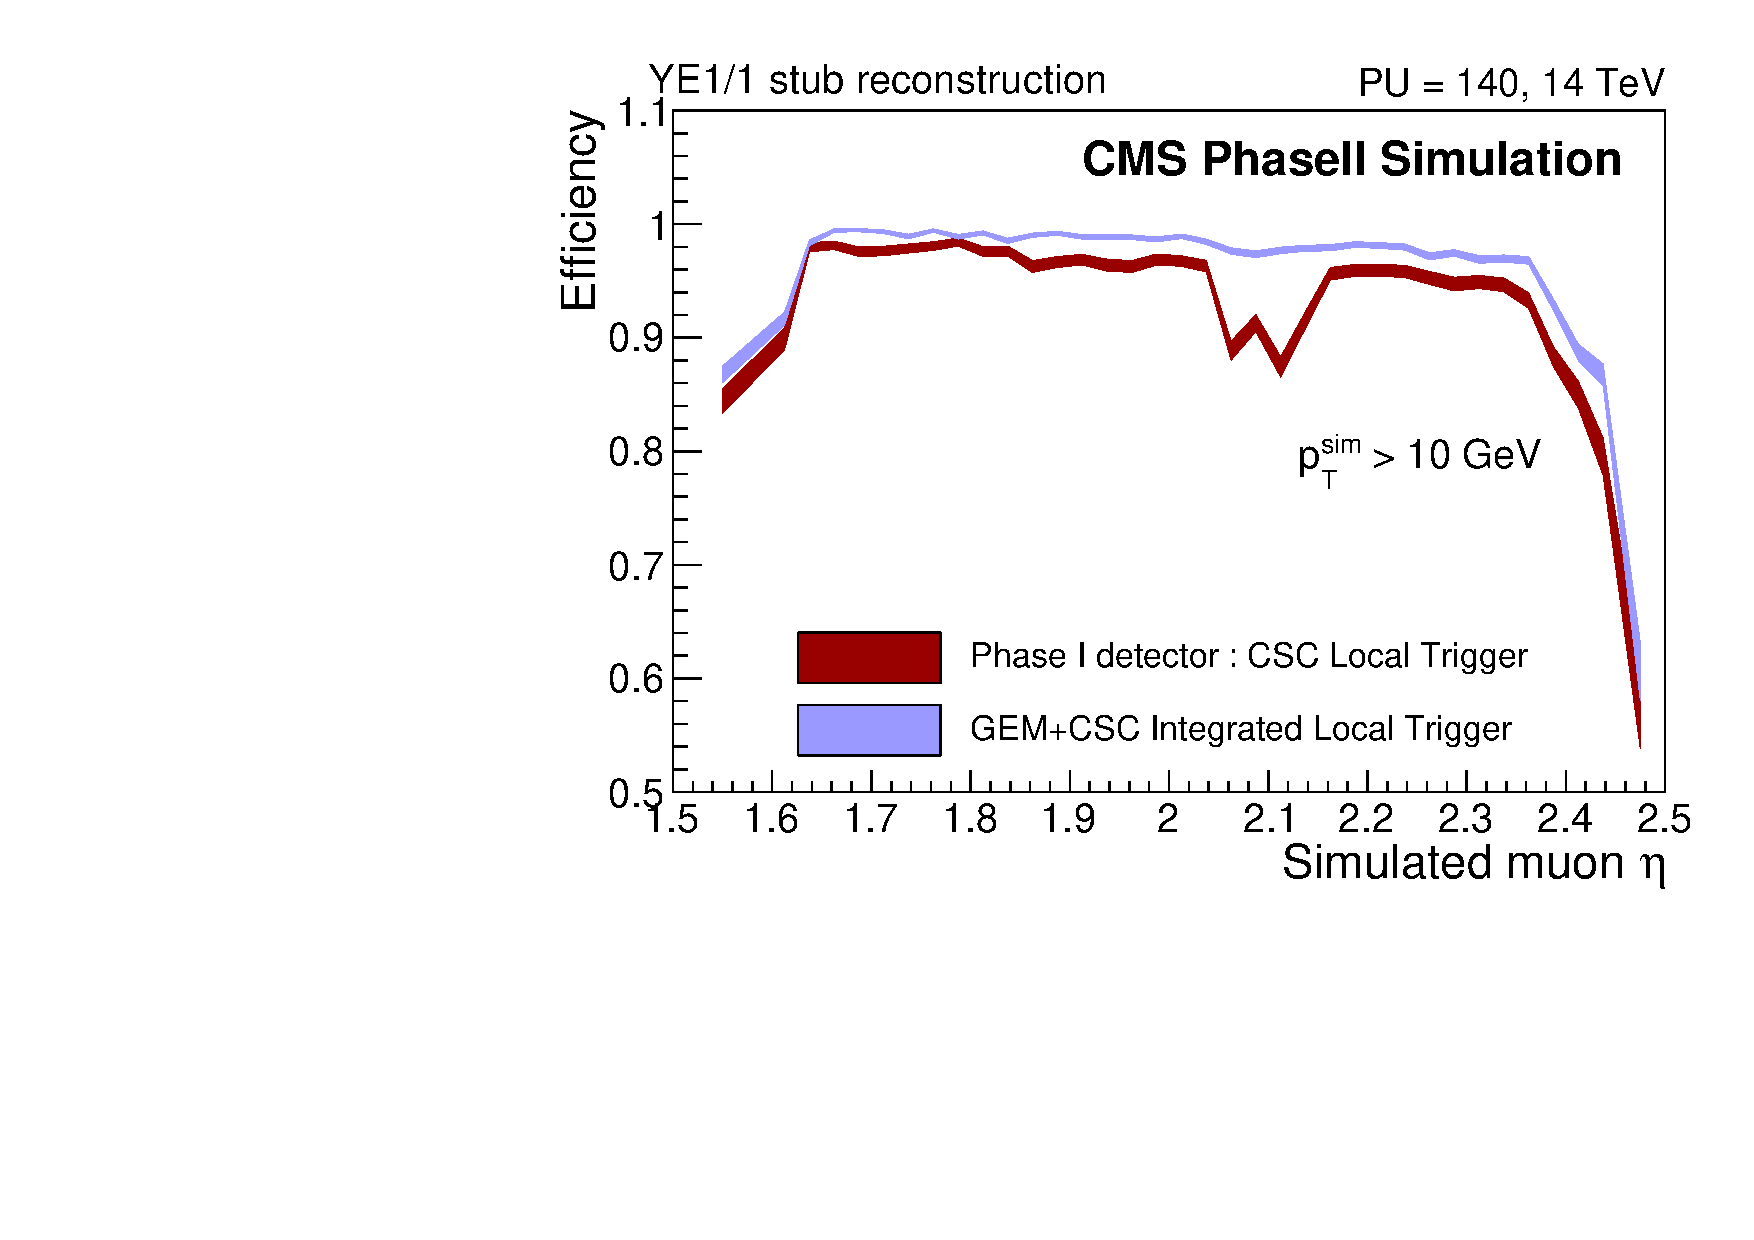
\includegraphics[width=\textwidth]{img/II-1-gem/gem-csc-efficiency.pdf}
      \caption{??? \cite{Colaleo:2021453}.}
      \label{fig:II-1-gem-trigger}
    \end{figure}

    Preserving a low p$_T$ threshold is essential for the physics analysis to preserve good reconstruction efficiency of soft muons. These particles are important for a wide range of processes from beyond the standard model searches to measurments in the Higgs sector. Simulation studies have shown that in the case of $ H \rightarrow \tau^+ \tau^- $ where one $ \tau $ decays into a muon, a decrease of 5 GeV c$^{-1}$ in the p$_T$ threshold results in an increase of 35\% in the acceptance of the channel. In addition, the impact is not limited to the single muon trigger but affects all other triggers involving muons analysing for example $\mu+jet$ or $e/\gamma+\mu$ signals. \\

    To further improve the trigger efficiency of CMS, it is planned to add a new track trigger, a trigger system for the tracker, which would benefit from the high resolution of the subdetector. Forseen to be integrated during LS2, the system yields excellent results in the identification, reconstruction, and triggering of muons. However, due to the high occupancy of hits and the limited amount of computanional time alocated to the trigger, given approximations need to be done, degrading the results for certain physics channels. One of the assumptions made by the algorithms is that every particle originates from the interaction point. This has a significant impact on new physics processes involving hidden sectors of low interacting particles such as the decay of a Higgs into two neutralinos $ n $, which in turn create a so-called dark photon $ \gamma_d $
    \begin{equation}
      h \rightarrow 2 n_1 \rightarrow 2 n_d \gamma_d .
    \end{equation}
    The dark photon in turn decays into two muons which originate from a displaced vertex. Figure \ref{fig:II-1-gem-dark-photon} illustrates the limitations of the track trigger (red) to reconstruct muons in function of the distance between the vertex and the interaction point. Efficiency quickly drops to reach 0\% around 50 cm. The muon standalone trigger (blue) on the other hand is capable of reconstructing the track with high efficiency underlining the necessity of a preserving excellent trigger performances in the muon spectrometer.

    \begin{figure}[h!]
      \centering
      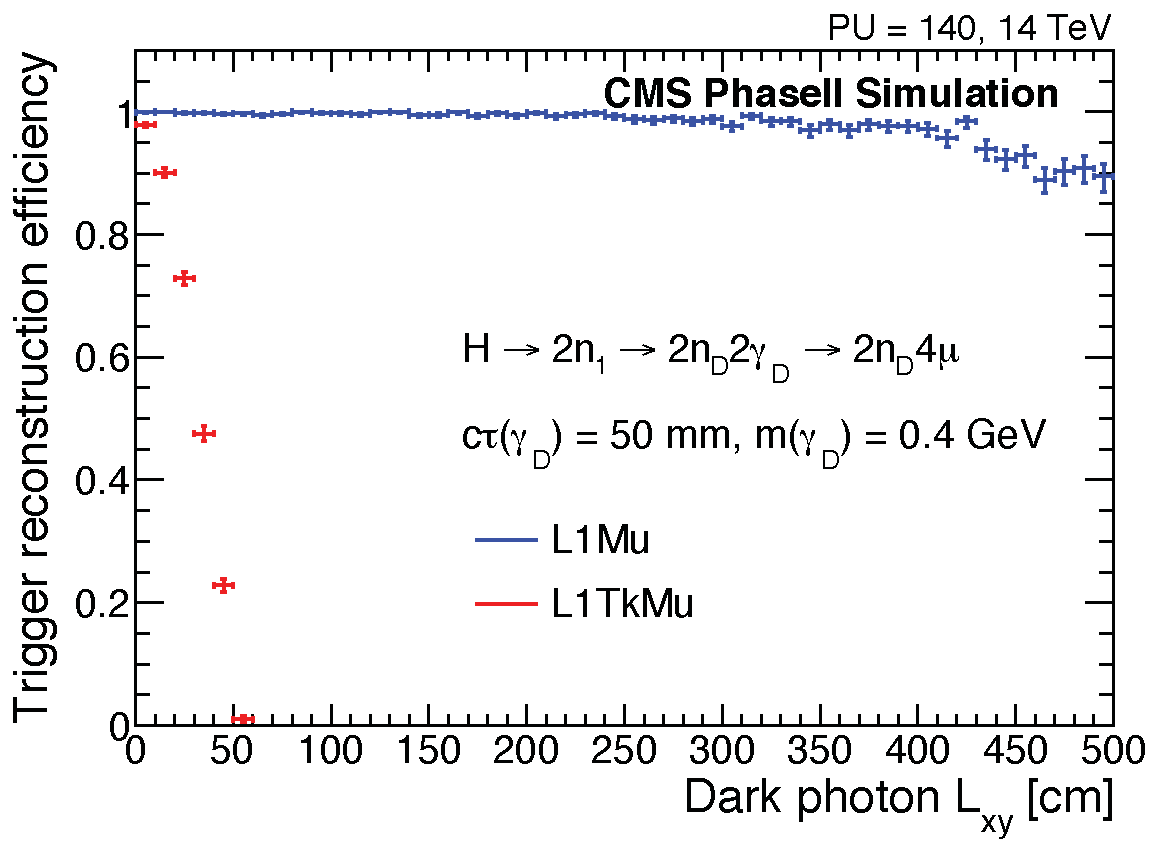
\includegraphics[width=0.6\textwidth]{img/II-1-gem/dark-photon.pdf}
      \caption{??? \cite{Colaleo:2021453}.}
      \label{fig:II-1-gem-dark-photon}
    \end{figure}

  \section{Technology Overview of Triple-GEM detectors}

    A GEM foil is a 50-$\mu$m-thick polymer foil covered with 5-$\mu$m-thin copper sheets on both sides chemically perforated by a high density of microscopic holes. The polymer used is either Kapton or Apical, both with a dielectric constant of 3.5. The holes are truncated double cones with an outer diameter of 70 $\mu$m and a inner diameter of 50 $\mu$m and are spaced by 140 $\mu$m on an hexagonal grid. The structure of the GEM foil as shown on the left in Figure \ref{fig:II-1-gem-holes}, is obtained using photolitography techniques that require precise aligment of the top and bottom masks. \\

    The diagram on the right in Figure \ref{fig:II-1-gem-holes} represents the electric field lines that appear when a high voltage difference is applied between the two layers of copper, typically on the order of 300 V, resulting in field densities inside the holes reaching approximatly 80 kV cm$^{-1}$. The structure of the electric field is used to amplify the signal of particles passing through the detector. Electrons resulting from the ionisation of the gas by charged particles are directed towards the holes of the foil. When reaching high kinetic energy inside the holes, they themselves ionize the medium, producing secondary avalanches of electrons. Each hole acts as a proportional counter with gains  \\

    \begin{figure}[h!]
      \centering
      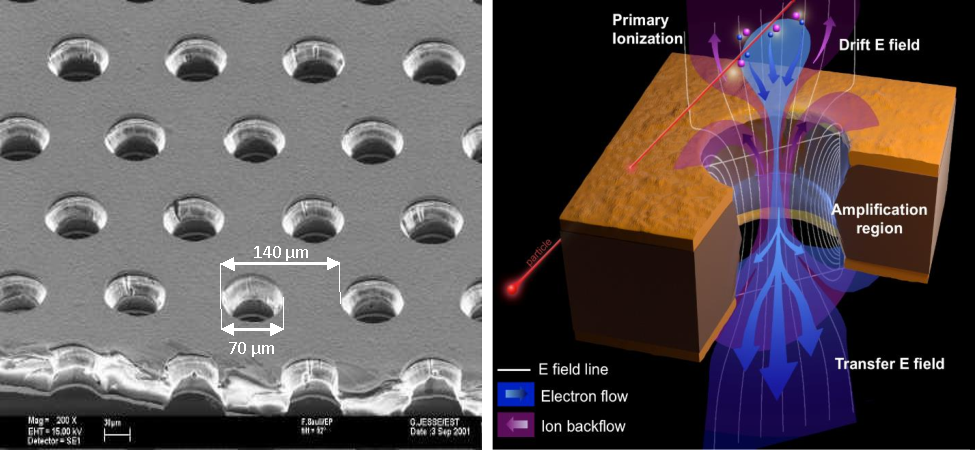
\includegraphics[width=\textwidth]{img/II-1-gem/holes.pdf}
      \caption{??? \cite{Colaleo:2021453}.}
      \label{fig:II-1-gem-holes}
    \end{figure}

    To achive high gains in the detectors, two solutions can be implemented: increase the high voltage on the foils, or use multiple foils. The first option gives rise to discharges when operating at too high electric fields thus damaging the detector. Therefore, the choice to use three GEM foils has been made, hence the name of Triple-GEM detectors. The foils are arrangend as shown in Figure \ref{fig:II-1-gem-triple}. A drift cathode is placed on the top of the chamber which creates an electric field between itself and the top copper layer of the first GEM foil in the so-called drift gap measuring 3 mm. Electrons originating from the ionisation of the ArCO$_2$ gas mixture (70\% Argon, 30\% CO$_2$) by a charged particle drift towards the holes of the foil, while ions are collected by the cathode. Following, the electron shower is amplified by GEM 1, GEM 2, and GEM 3, respectivly tranfering the signal to the transfer 1, transfer 2, and induction gaps measuring 1 mm, 2 mm, and 1 mm each. The size of each gap is of importance in the detector performance and has been optimized over time to increase the speed of the signal and the detector efficiency. The current configuration is called 3/1/2/1 mm in reference to the gap size. In the induction gap, the drift of the electrons towards the anodes induces a signal on the latter which can be detected by electronics. \\

    \begin{figure}[h!]
      \centering
      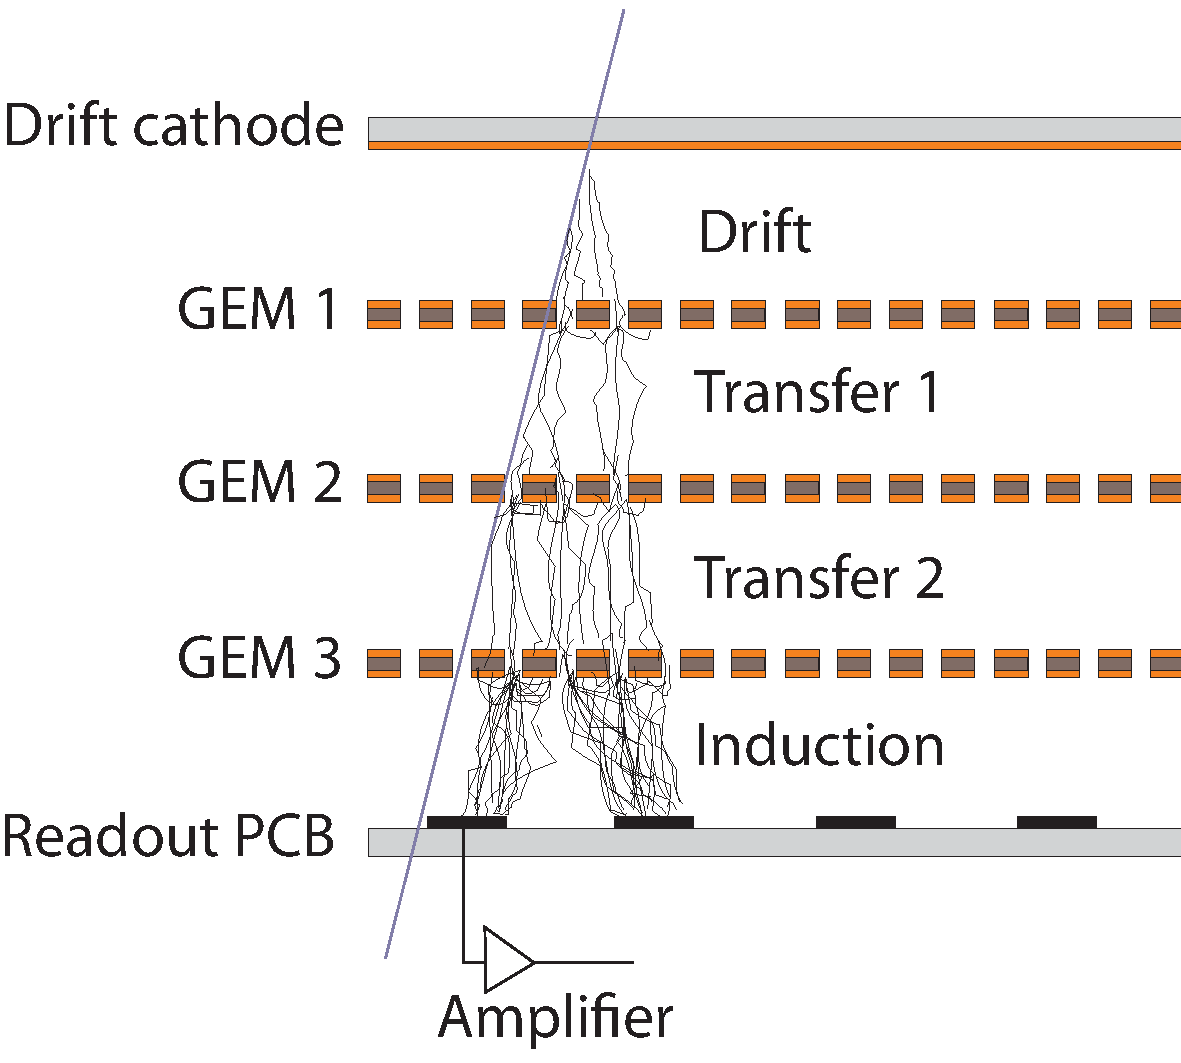
\includegraphics[width=0.5\textwidth]{img/II-1-gem/triple-gem-foils.pdf}
      \caption{??? \cite{Colaleo:2021453}.}
      \label{fig:II-1-gem-triple}
    \end{figure}

  \section{Technical Design of GE1/1 chambers for CMS}

    The GE1/1 chambers are arranged in pairs to form superchambers, each covering 10$^o$ in $ \phi $ for a total of 72 chambers per endcap. The geometry of the superchambers is represented in Figure \ref{fig:II-1-gem-superchamber}. Due to mechanical constraint, the trapezoidal chambers are declined in two versions: a short one and a long one. The short chambers cover 1.61 < |$\eta$| < 2.18 and have a large base of 445 mm, a small base of 220 mm, and a height of 990 mm. The long chamers cover 1.55 < |$\eta$| < 2.18 and have a large base of 510 mm, a small base of 279 mm, and a height of 1283 mm. \\

    \begin{figure}[h!]
      \centering
      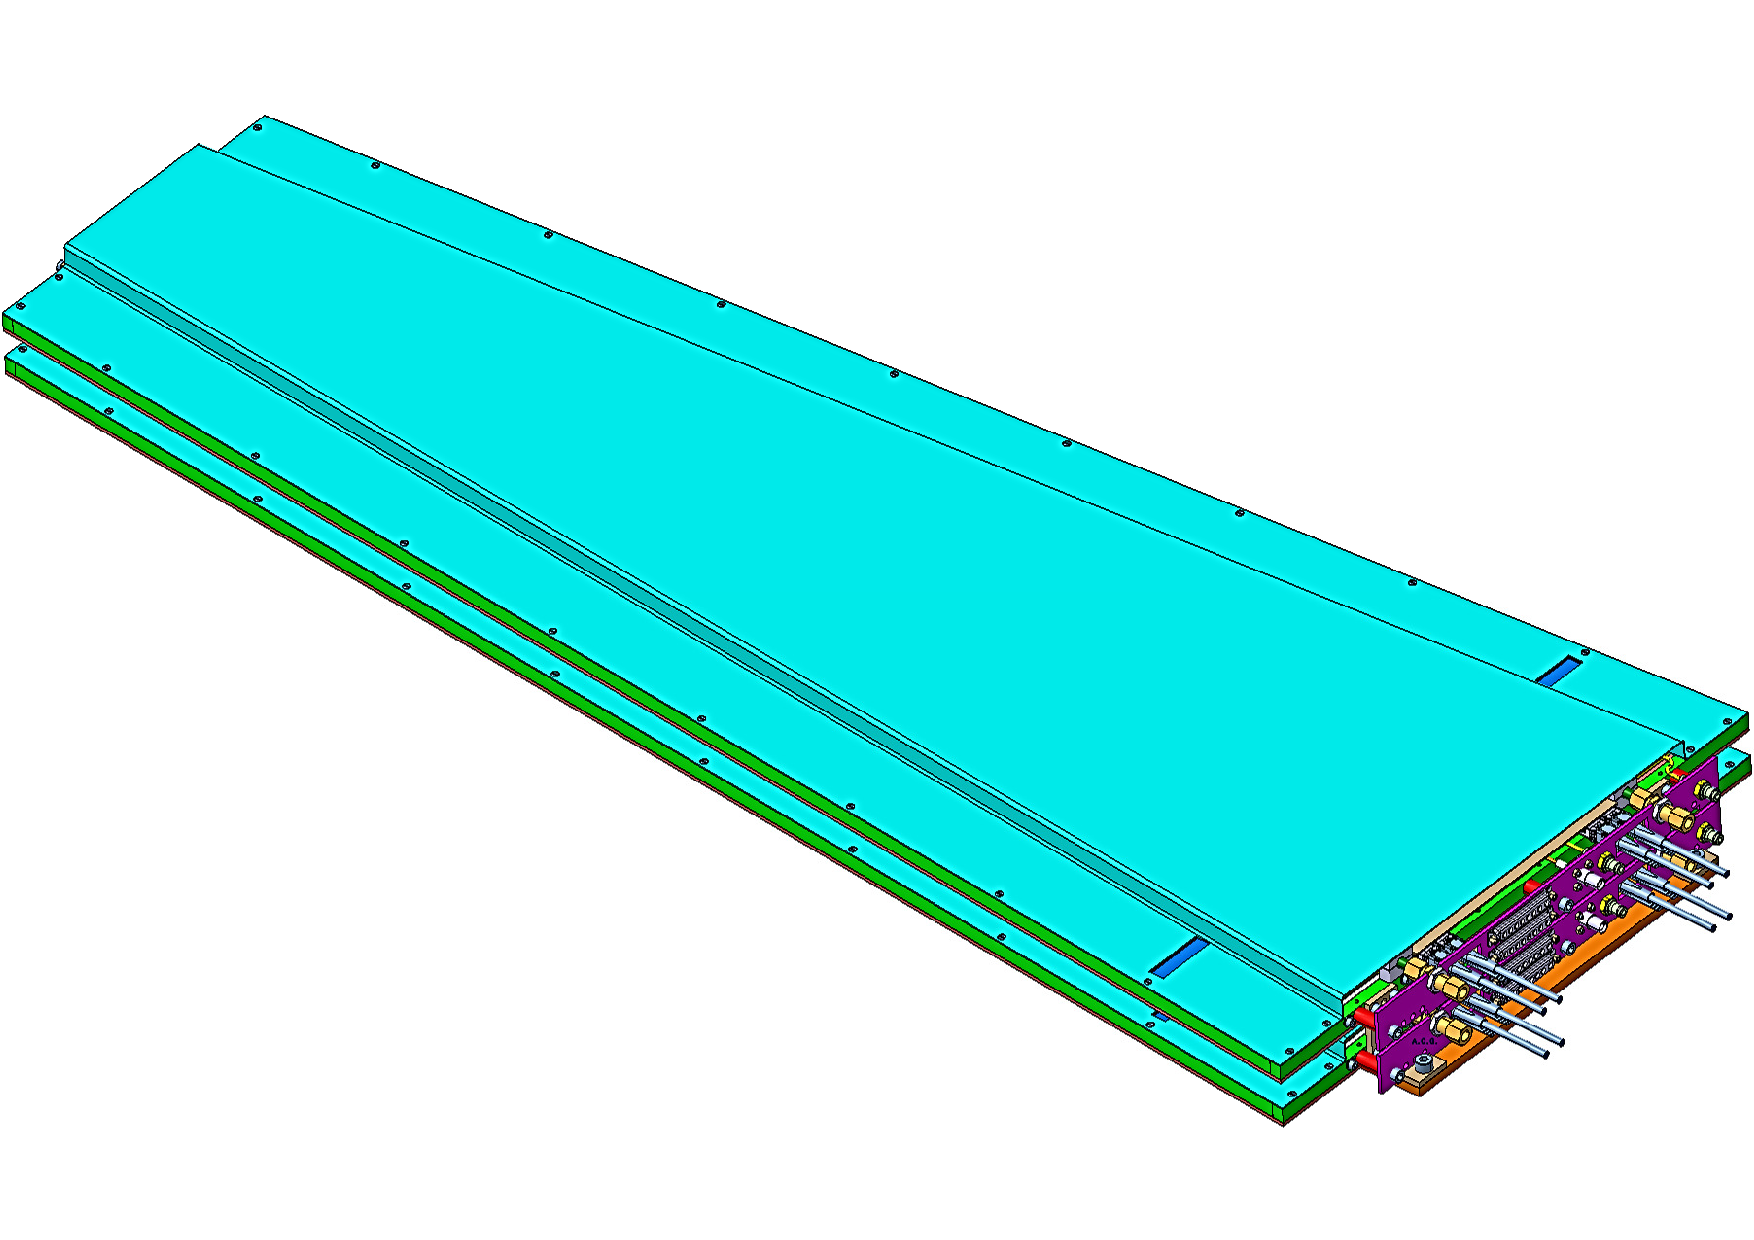
\includegraphics[width=0.6\textwidth]{img/II-1-gem/superchamber.pdf}
      \caption{??? \cite{Colaleo:2021453}.}
      \label{fig:II-1-gem-superchamber}
    \end{figure}

    The structure of a single chamber is shown in Figure \ref{fig:II-1-gem-exploded}. The drift cathode is placed on the bottom of the detector on which a frame is attached. The three GEM foils are streched out using screws embedded in the frame along with the seals making the chamber air tight. The anode strips are engraved on the readout board that closes the active region of the detector. One chamber is divided into three $ \phi $ sectors and eight $ \eta $ sectors with 128 strips running radially in each. This results in a mean coverage per strip of 450 $\mu$rad and a pitch varying from approximatly 500 $\mu$m to 1.3 mm. To each group of 128-strips a front-end electronics chip called the VFAT2 is attached. It digitizes the signals from the strips returning a single hit/not-hit bit. The VFAT2s are all connected to the GEM Electronics Board (GEB) which acts as router to forward the data towards the OptoHybrid (OH), a concentrator board located on the large side of the GEM which is the interface to the off-detector electronics. The VFAT2s and the OH are cooled down using cooling pipes attached on the top of the boards. Finally, a protective cover closes and protects the detector. When two chambers are assembled, a patch pannel is added in order to facilitate the insertion and removal of the low and high voltage cables, the water for the cooling, the gas, and the optical fibres connected to the DAQ system. Note that a signel source of high voltage is needed to power a chamber thanks to the use of a ceramic voltage divider which spreads the voltage over the various layers. \\

    \begin{figure}[h!]
      \centering
      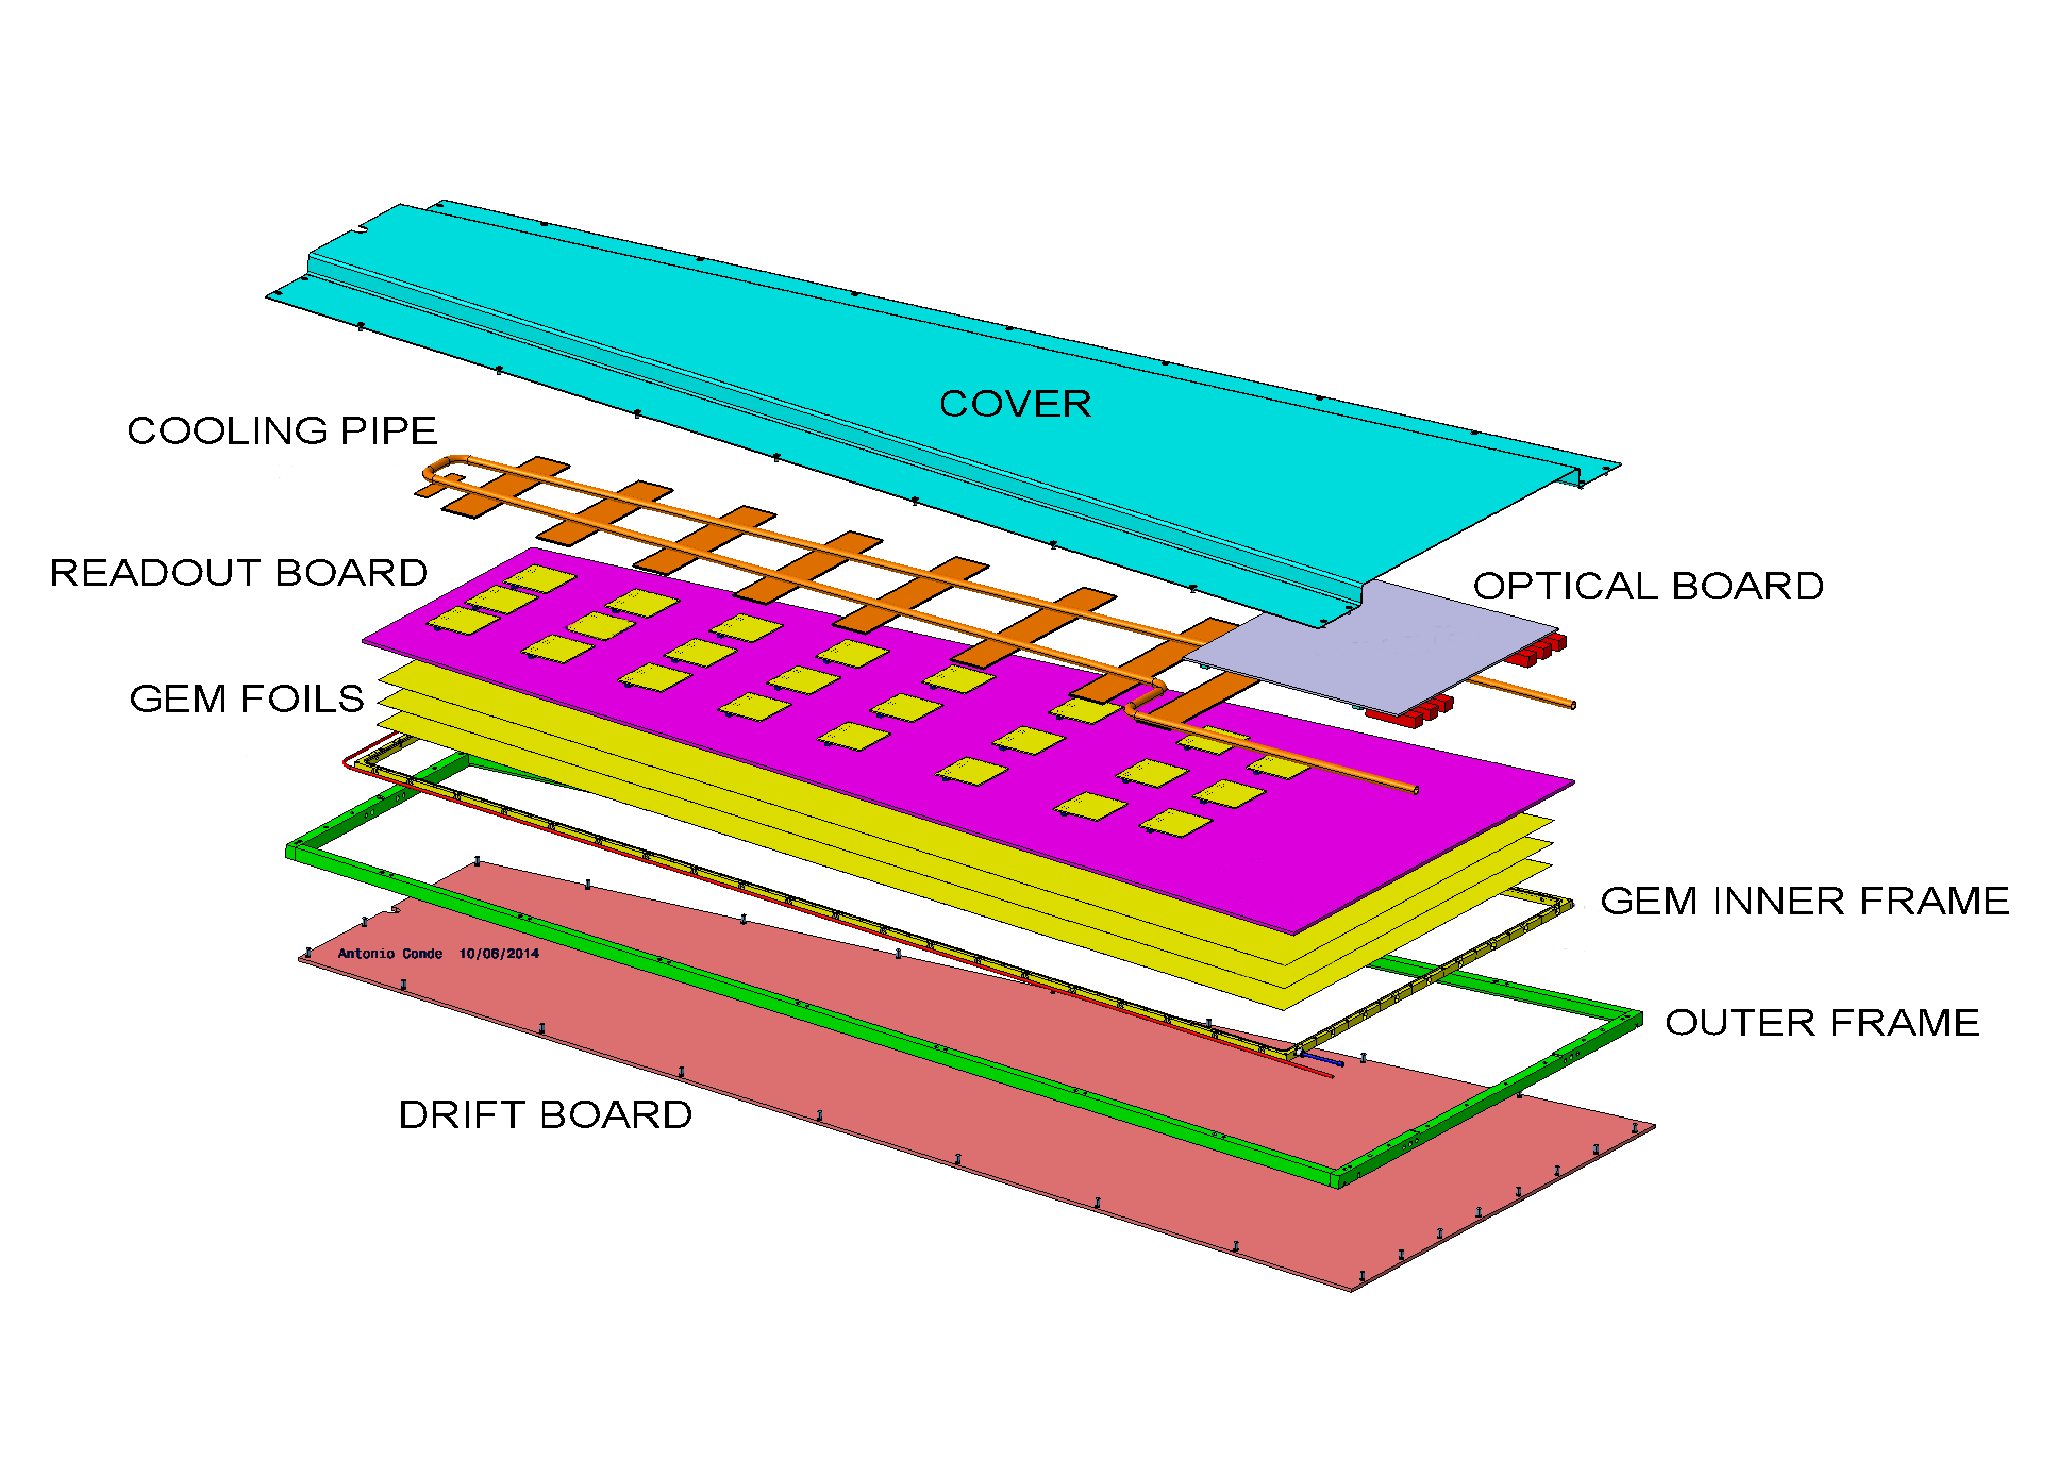
\includegraphics[width=\textwidth]{img/II-1-gem/gem-exploded.pdf}
      \caption{??? \cite{Colaleo:2021453}.}
      \label{fig:II-1-gem-exploded}
    \end{figure}

    Once assembled, the 72 superchambers will be installed in the endcaps of CMS as displayed in Figure \ref{fig:II-1-gem-wheel}. The full ring will be placed in the so-called nose of the endcap, between the HCAL and the ME1/1 stations.

    \begin{figure}[p]
      \centering
      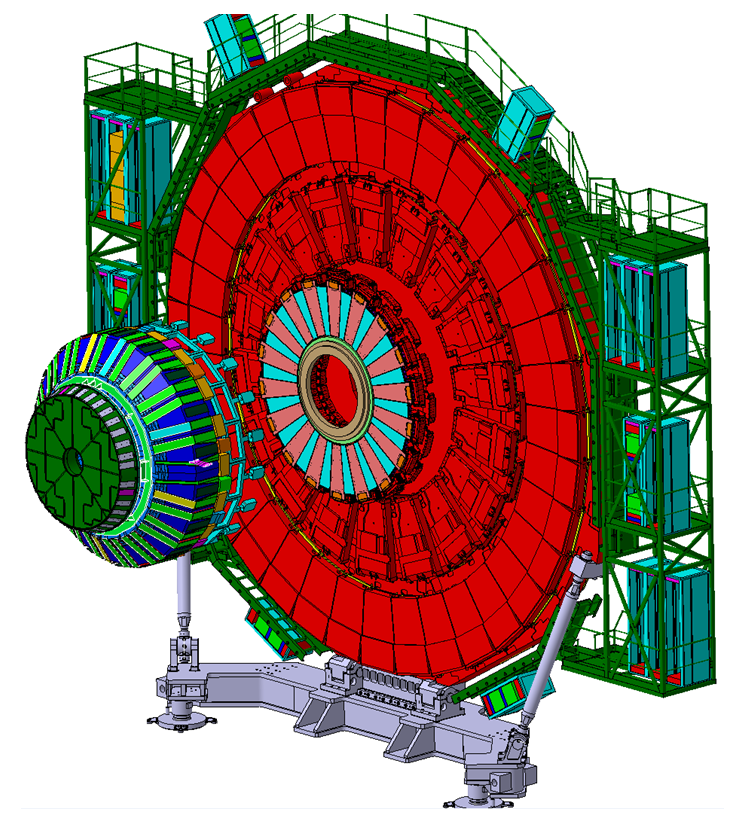
\includegraphics[width=\textwidth]{img/II-1-gem/wheel.png}
      \caption{??? \cite{Colaleo:2021453}.}
      \label{fig:II-1-gem-wheel}
    \end{figure}

  \section{Detector Design Evolution}

    The design and fabrication method of the GE1/1 chambers has evolved over the past 5 years of R\&D. The five generations of detectors are shown in Figure \ref{fig:II-1-gem-generations}. GE1/1-I was the first 1-m-long prototype. It was equipped with only eight readout sectors, components were glued together and GEM foils were separated using spacers. The number of sectors was increased to 24 in GE1/1-II with the full granularity of the current design (384 strips per 10$^o$). The gap configuration was changed from 3/2/2/2 mm to 3/1/2/1 mm to increase the signal speed. From GE1/1-III and onwards, GEM foils were streched mechanically using an outer frame glued on the drift board. This design also introduced the use of a miniature ceramic high voltage divider to apply voltage on the foils. However, the assembly of the chamber induced mechanical tension on the readout board, deforming the detector and resulting in a non-uniform response. This problem was resolved in GE1/1-IV by pre-bending the boards in the opposite direction to compensate before being bolted to the frames. This geneation was the first assembled without glue, reducing production time to a few hours. However, the pre-beding technic did not yield viable results. Therefore, GE1/1-V uses pull-out pieces to tension the foils to the outer frame, on which the drift and readout board are bolted. The outer frame serves as a wall for the chamber and seales it using O-rings. Finally, the version of the design of the chambers that will be installed in CMS is GE1/1-VI which has optimized dimension to maximize the geometrical acceptance.

    \begin{figure}[h!]
      \centering
      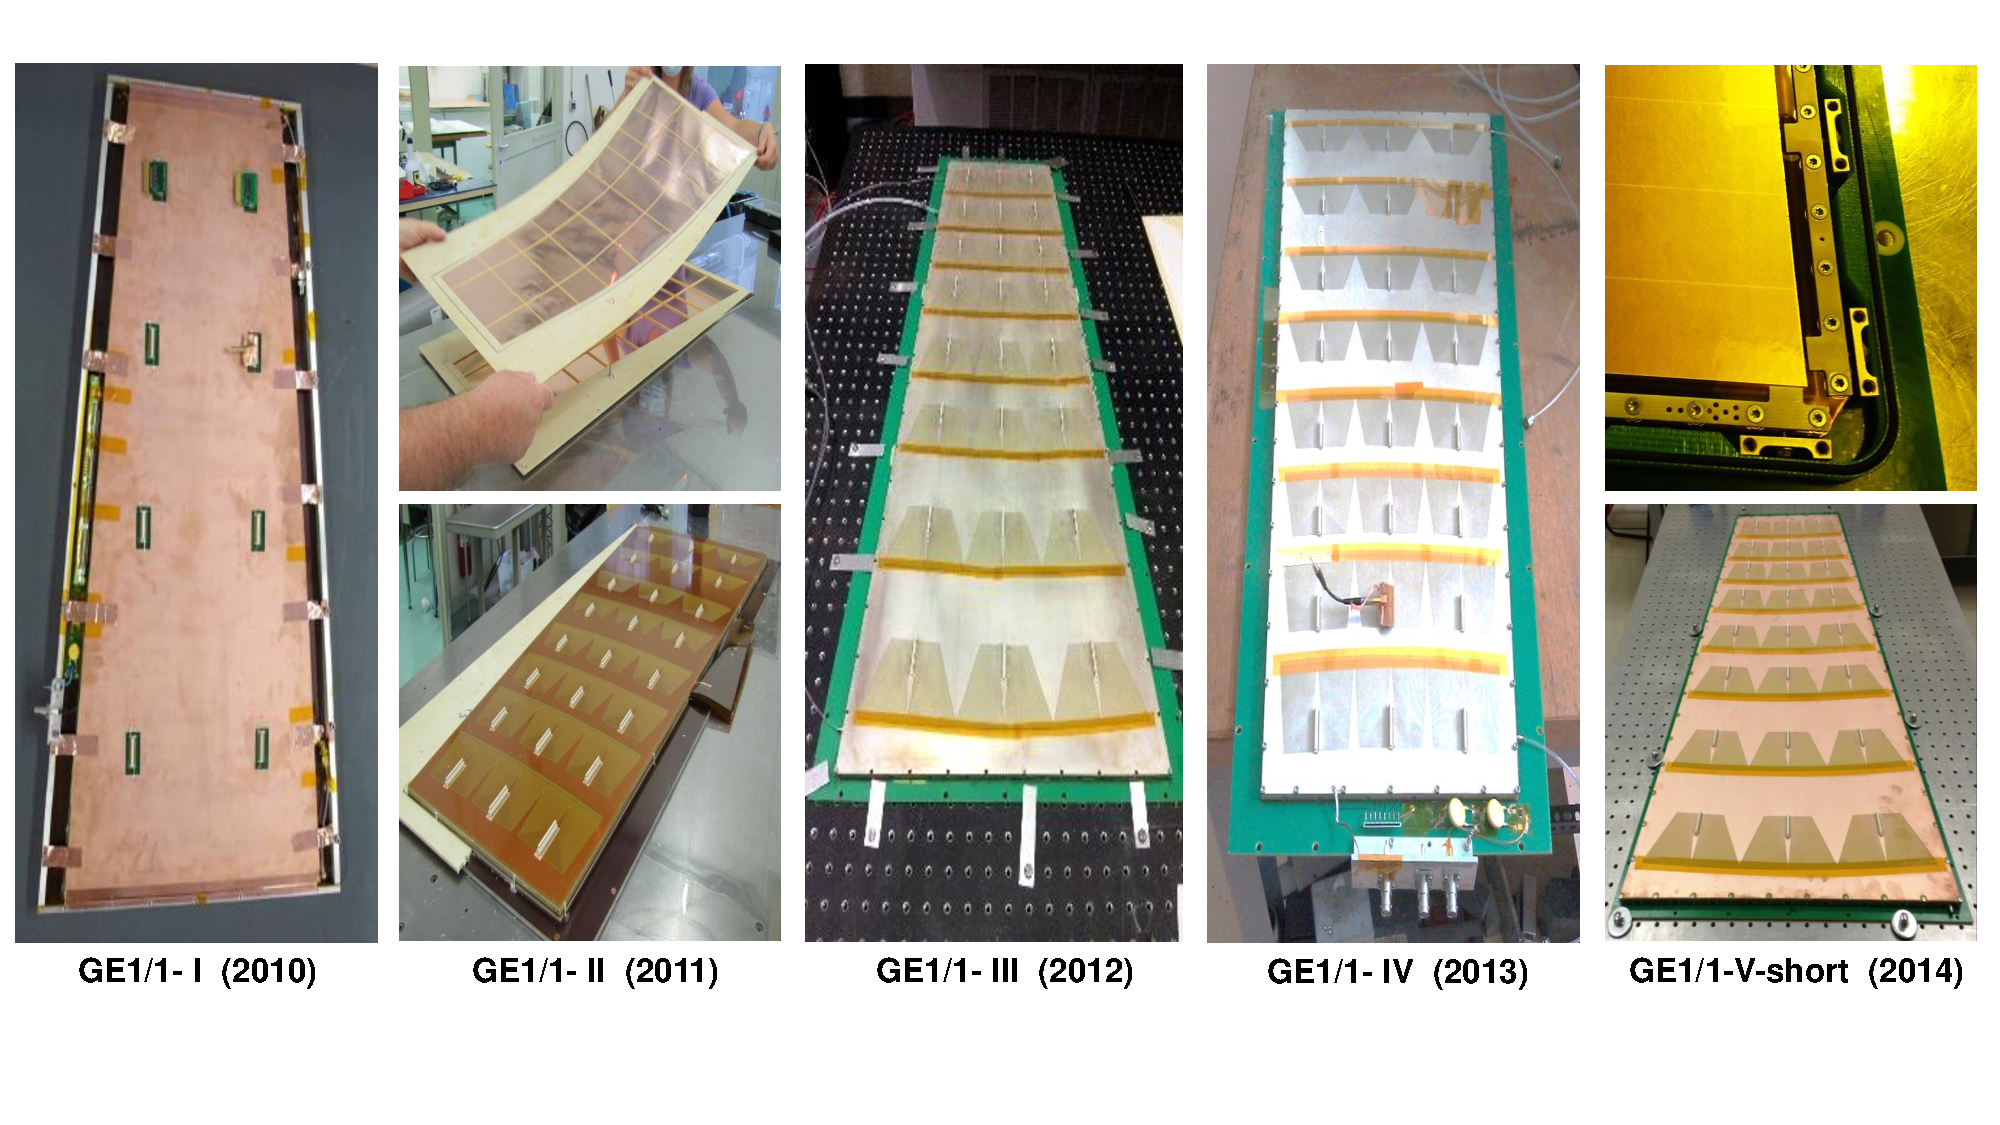
\includegraphics[width=\textwidth]{img/II-1-gem/generations.pdf}
      \caption{??? \cite{Colaleo:2021453}.}
      \label{fig:II-1-gem-generations}
    \end{figure}

  \section{GE1/1 Prototyping Results}

    In order to provide the desired trigger and physics performance, the GE1/1 chambers must meet the following list of requirements:
    \begin{itemize}
      \item Maximum geometric acceptance within the given CMS envelope;
      \item Rate capability of 10 kHz cm$^{-2}$ or better to cope with the HL-LHC hit rate;
      \item Single-chamber efficiency of 97\% or better for detecting minimum ionizing particles resulting in 99.9\% efficiency for a superchamber when signals are combined with a logical OR;
      \item Angular resolution of 300 $\mu$rad or better on $ \Delta \phi = \phi_{GE1/1} - \phi_{ME1/1} $ to discriminate high-p$_T$ from low-p$_T$ muons;
      \item Timing resolution of 10 ns or better for a single chamber, which can be improved when combining the superchamber measurments, to allow matching with the CSC hits;
      \item Gain uniformity of 15\% or better across a chamber and between chambers to ensure that no geometrical or trigger biases are present. \\
    \end{itemize}

    These features have been tested during test beam campaigns on the GE1/1 prototypes using the APV25 front-end chips to provide an analog readout of the detector.
































  \section{GEM Upgrade Schedule}
